\section{Validating graphs}\label{sec:valGraph}

In the previous section, we described an algorithm to verify proof trees. Proofs trees are a very natural way to encode certificates for datalog results but have some drawbacks. 

\begin{example}\label{ex:treeGraph}
    Consider the following program that computes the transitive closure in a different way.

    \begin{equation}
        \begin{split}
            T(?x,?y) &\leftarrow E(?x,?y). \\
            T(?x,?z) &\leftarrow T(?x, ?y), T(?x, ?y), E(?y, ?z). \\
        \end{split}
    \end{equation}

    The database shall encode the elements of a chain $E(i, i+1)$ for $i \in \{0, n\}$. In the proof tree representation we need the same proof tree twice for $T(?y, ?z)$ in the second rule and will need copies for it later, which results in large trees. The proof tree for $T(0, i+1)$ needs a node for this fact, one for the $E$ fact $E(i, i+1)$ and two proof trees for $T(0, i)$. Therefore the size of $T(0, i+1)$ in the number of nodes is more than double the size of $T(0, i)$ which leads to an exponential growth.
\end{example}

Proof trees offer no reusability as they need to stay in the tree shape. Formally we can view the proof tree as a tree $T= (V_T;E_T)$ with a label function $label: V_T \to groundAtom$ because different vertices have the same label in a proof tree as in the example above.

A more compact representation would be a directed graph $G=(V_G, E_G)$ of $T$  with $V_G = \{a \mid \exists v \in V_T, label(v)=a\}$ and $E_G = \{ (a_1, a_2) \mid \exists v_1, v_2 \in V_T,  label(v_i) = a_i \land (v_1, v_2) \in E_T\}$. Then a vertice can be considered equal to its label as no label occurs multiple times anymore. Examples for a proof tree and the corresponding graph are in \cref{fig:treeGraph}.


\begin{figure}
  \centering
  \begin{subfigure}[b]{0.65\textwidth}
    \centering
    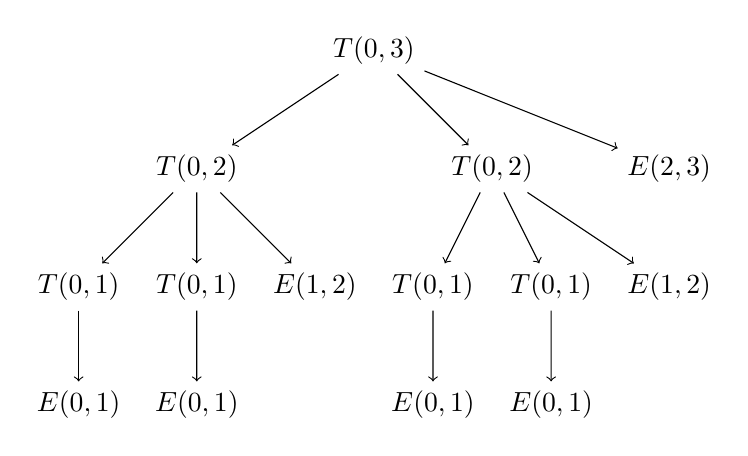
\begin{tikzpicture}[scale=.75]
      \node (A) at (5,4) {$T(0,3)$};

      \node (B) at (2,2) {$T(0,2)$};
      \node (C) at (7,2) {$T(0,2)$};
      \node (D) at (10,2) {$E(2,3)$};

      \node (E) at (0,0) {$T(0,1)$};
      \node (F) at (2,0) {$T(0,1)$};
      \node (G) at (4,0) {$E(1,2)$};
      \node (H) at (6,0) {$T(0,1)$};
      \node (I) at (8,0) {$T(0,1)$};
      \node (J) at (10,0) {$E(1,2)$};

      \node (K) at (0,-2) {$E(0,1)$};
      \node (L) at (2,-2) {$E(0,1)$};
      \node (M) at (6,-2) {$E(0,1)$};
      \node (N) at (8,-2) {$E(0,1)$};

      \draw[->] (A) -- (B);
      \draw[->] (A) -- (C);
      \draw[->] (A) -- (D);
      \draw[->] (B) -- (E);
      \draw[->] (B) -- (F);
      \draw[->] (B) -- (G);
      \draw[->] (C) -- (H);
      \draw[->] (C) -- (I);
      \draw[->] (C) -- (J);
      \draw[->] (E) -- (K);
      \draw[->] (F) -- (L);
      \draw[->] (H) -- (M);
      \draw[->] (I) -- (N);
    \end{tikzpicture}
    \caption{A proof tree for $T(0,3)$}
    \label{fig:proofTree}
  \end{subfigure}
  \hfill
  \begin{subfigure}[b]{0.25\textwidth}
    \begin{tikzpicture}
      \node[circle] (A) at (0,4) {$T(0,3)$};
      \node[circle] (B) at (-1,2) {$T(0,2)$};
      \node[circle] (C) at (2,2) {$E(2,3)$};
      \node[circle] (D) at (-1,0) {$T(0,1)$};
      \node[circle] (E) at (2,0) {$E(1,2)$};
      \node[circle] (F) at (-1,-2) {$E(0,1)$};

      \draw [->] (A) -- (C);
      \draw[->] (A) to[out=235, in=150] (B);
      \draw[->] (A) to[out=280, in=45] (B);
      \draw [->] (B) -- (E);
      \draw[->] (B) to[out=235, in=150] (D);
      \draw[->] (B) to[out=280, in=45] (D);
      \draw[->] (D) -- (F);
    \end{tikzpicture}
    \caption{A proof graph for $T(0,3)$}
    \label{fig:proofGraph}
  \end{subfigure}
  \caption{An example of a proof tree and a proof graph for the same fact from \cref{ex:treeGraph}}
  \label{fig:treeGraph}
\end{figure}

Another advantage occurs when we want to validate multiple trees or even a complete result. Multiple trees will often share labels as well and combining them into a graph, i.e. the union of $G_{T_i}$ for trees $T_i$ will again include every label just once. In the previous section, we introduced the possibility of not having to check every proof tree as they occur in other proof trees as well. Selecting a minimal amount of proof trees to check a complete result is however still an instance of the NP-hard subset cover problem.

We require for this that if the successors of a ground atom are the same elements  in every tree if the ground atom occured in this tree. If not an atom would have more successors then previously in the tree and probably no matching ground rule. In practice, this requirement was always fulfilled.

Another requirement is acyclicity. We cannot use an atom to explain itself. Either we could have used it directly before or it cannot be explained by a proof tree at all. 
\subsection{Graph model}

As a number of different results from mathematics are already formalized in mathlib, it is no surprise that graphs are already modelled in mathlib as depicted below:

\begin{lstlisting}
structure SimpleGraph (V : Type u) where
  /-- The adjacency relation of a simple graph. -/
  Adj : V → V → Prop
  symm : Symmetric Adj 
  loopless : Irreflexive Adj
\end{lstlisting}

This graph representation is unfortunately not what we need in an algorithm. Firstly, the adjacency relation of this graph is always symmetric so that it does not encode the directed graphs we need. Secondly, the adjacency relation is a function to \lstinline|Prop| and thus in general not computable but we want to use it in an algorithm. Finally, we need for the validation the successors of a vertex as they are supposed to represent the body of a ground rule. When we want to get them in this model we would have to ask the adjacency relation for every vertex if it would be computable.

Therefore we design our own implementation of a graph. We use an adjacency list approach so that we can quickly get all the successors of a vertex. This represented by a hash map whose keys are the vertices. Each vertex is mapped via the hash map towards its successors.

\begin{lstlisting}
    abbrev (.\PreGraph.) (A: Type) [DecidableEq A] [Hashable A] := 
        Std.HashMap A (List A)

    def (.\PreGraphvertices.) (g : PreGraph A) : List A := g.toList.map Prod.fst
    def (.\PreGraphsuccessors.) (g : PreGraph A) (a : A) : List A := g.findD a []
\end{lstlisting}

\lstinline|Std.HashMap.toList| returns here a list of pairs of the type $(A, List\ A)$, i.e. a vertex and its successors. Using \lstinline|Prod.fst| we obtain the first element of every pair in the list, which are all vertices. \lstinline|Std.HashMap.findD a []| returns the value saved with $a$ in the hash map which are the successors of $a$. If a vertex is not present (the value is not in the hash map), then $[]$ is returned which is the fall back option provided to  \lstinline|Std.HashMap.findD|.

This approach contains all important elements in a graph, but there is a small technical problem with it. 

\begin{example}
    
    Consider the graph depicted in \cref{ex:counterexampleGraph}. An element is colored, if it is in the list of vertices. The successors of a vertice are all elements that 

\begin{figure}
    \centering
    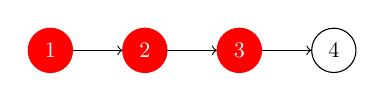
\begin{tikzpicture}[scale=0.8,transform shape]
        % Define styles for nodes and edges
        \tikzstyle{vertex}=[circle, draw=black, fill=white, minimum size=20pt, inner sep=0pt]
        \tikzstyle{rednode}=[vertex, red]
      
        % Define vertices
        \node[rednode] (v1) at (1.5,0) {\textcolor{white}{1}};
        \node[rednode] (v2) at (3,0) {\textcolor{white}{2}};
        \node[rednode] (v3) at (4.5,0) {\textcolor{white}{3}};
        \node[vertex] (v4) at (6,0) {4};
      
        % Draw edges
        \draw[->] (v1) -- (v2);
        \draw[->] (v2) -- (v3);
        \draw[->] (v3) -- (v4);
      
      \end{tikzpicture}
    \caption{An example of a pregraph}      
    \label{ex:counterexampleGraph}

\end{figure}
    We can view the type \lstinline|Fin 5|, i.e. the natural numbers $n$ with the property that $n<5$. The vertices are the list $[1,2,3]$. The vertex 3 has the element 4 as a successor, but 4 is not a vertex of the graph. Such a behaviour is undesireable as searching for vertices that satisfy some criteria may lead outside of the graph.
\end{example}

We define a pregraph to be complete, if every successor of a vertex is a vertex itself and can then avoid the problem.

\begin{lstlisting}
    def (.\PreGraphcomplete.) (pg: PreGraph A) := 
    ∀ (a:A), pg.contains a →  ∀ (a':A), a' ∈ (pg.successors a) → pg.contains a'
\end{lstlisting}

A graph is then a complete pre-graph and we can lift all previous operations to this new type.
\begin{lstlisting}
abbrev (.\Graph.) (A: Type) [DecidableEq A] [Hashable A] := 
    { pg : PreGraph A // pg.complete }
\end{lstlisting}

The completeness predicate was necessary, because our type is a superset than the vertices that occur in the graph. We do not expect every ground atom to be in the graph. An alternative would be to create a subtype of those ground atoms that occur in a list but this requires many types conversions when creating a graph from scratch as the list of vertices will change. Here we can add vertices to the graph and only have to prove that the completeness property still holds at the end.

We start by formalizing walks in a graph. Walks allow the repitition of vertices in itself in contrast to paths which suffices us.

A walk $w$ in a graph $G$ is a list of vertices that are all vertices of $G$ and are connected via the successor relation of $G$, i.e. for every $i$ with $0 < i < i.length$ we have that $w[i-1] \in G.successors\ w[i]$. The starting vertex of the walk is consequently at the back.

\begin{lstlisting}
def (.\isWalk.) (l: List A) (G: Graph A): Prop :=
    (∀ (a:A), a ∈ l → a ∈ G.vertices ) ∧ 
    ∀ (i: ℕ), i > 0 → ∀ (g: i < l.length), l.get (Fin.mk i.pred (pred_lt i l.length g)) ∈ G.successors (l.get (Fin.mk i g) )
\end{lstlisting}

The \lstinline|pred| function returns the predecessor of any natural number that is not zero and zero otherwise. Because we use the \lstinline|List.get| function we not only have to specify a position but also a proof that this position is smaller than the length of the list to not get an error. These two elements are combined into a Fin type. In the future we usually omit these proofs in this work because of the length.

Due to the completeness predicate it would suffice to require that the starting vertex is in $G$ but this variant is simpler to state. We also allow the empty walk $[]$ as this will be beneficial in later applications.

Lists are beneficial in this use case in contrast to arrays because they can easily be extended at the front which we will use when explore a graph algorithmically. We can always extend a walk by a successor of the leading element.

\begin{lemma}[\isWalkextendssuccessors]
    Let $w$ be a list of vertices and $a$ and $b$ be vertices.
    If $a::w$ is a walk in $G$ and $b$ is a successor of $a$ in G then $b::a::w$ is also a walk in $G$.
\end{lemma}

A cycle is supposed to be a walk that starts and ends with the same node and an acyclic graph is a graph that has no cycles. As any list that only contains a single vertex of the graph would fulfill this property we require that a cycle has additionally at least length two.

\begin{lstlisting}
def (.\isCycle.) (l: List A) (G: Graph A): Prop :=
  if h: l.length < 2
  then False
  else

  isWalk l G ∧ l.get (Fin.mk 0 _) = l.get (Fin.mk l.length.pred _)

def (.\isAcyclic.) (G: Graph A) := ∀ (l: List A), ¬ isCycle l G
\end{lstlisting}

\subsection{Validation of a graph}

After defining the graph model, we want to specify how the graph validation takes place. For these we defined the recursive predicate \isValid and implemented it using \treeValidator. As the graph we receive may not even be acyclic we cannot simply define a recursive predicate as this will then not terminate. Instead we define a local predicate for each vertex and its successor. Then we can check every vertex individually.

\begin{lstlisting}
def (.\locallyValid.) (P: program τ) (d: database τ) (v: groundAtom τ) (G: Graph (groundAtom τ)): Prop :=
 (∃(r: rule τ) (g:grounding τ), r ∈ P 
    ∧ ruleGrounding r g = {head:= v, body:= (G.successors v) }) 
 ∨ ((G.successors v) = [] ∧ d.contains v)
\end{lstlisting}

Except for the recursive case this is very similar to \isValid. Therefore we can reuse earlier concepts and build a checker for this. We expect the program again parsed into a look-up structure $m$, a database $d$, the vertex $a$ and its successors passed as a list $l$.

\begin{lstlisting}
def (.\localValidityCheck.) (m: List τ.predicateSymbols → List (rule τ)) (d: database τ) (l: List (groundAtom τ)) (a: groundAtom τ) : Except String Unit :=
  if l.isEmpty
  then
    if d.contains a
    then Except.ok ()
    else checkRuleMatch m (groundRule.mk a l)
  else
    checkRuleMatch m (groundRule.mk a l)
\end{lstlisting}

The correctness is proven similar as before assuming that $m$ is the result of \parseProgramToSymbolSequenceMap of the program $P$.

\begin{lemma}[\localValidityCheckUnitIffLocallyValid]
    Let $d$ be a database and $P$ be a program. If $m$ is the result of \parseProgramToSymbolSequenceMap with a function that maps any element to the empty list and $l$ is the list of successors of a ground atom $a$. Then the \localValidityCheck returns ok iff $a$ is locally valid with respect to $P$ and $d$.
\end{lemma}

In the next section we will show a method to show that a graph is acyclic and all elements are locally valid with respect to $P$ and $d$. In the remainder of this section we assume that this is true and devise a method to show that then all vertices of the graph are in the proof-theoretic semantics of $P$ and $d$.

Our goal is to create a proof-tree for every node. We devise a function that creates such a proof tree for a given node by recursively calling it on the successors.

\begin{lstlisting}
def (.\extractTree.) (a: A) (G: Graph A) (mem: a ∈ G.vertices) (acyclic: isAcyclic G): tree A :=
  tree.node a (List.map (fun ⟨x, _h⟩ => extractTree x G (G.complete a mem x _h) acyclic) (G.successors a).attach)
\end{lstlisting}

This function only terminates because the graph is acyclic. Therefore we require the fact as an explicit argument in the function above. We will argue with the vertices that are reachable from a vertex. These decrease the further we walk in the graph or else we would be able to reach a previous node and have a cycle which is not allowed. We start by formalizing the notion of reachability. We say that a vertex $a$ \canReach a vertex $b$ if there exists a walk $w$ from $a$ to $b$. (The start of the walk is the last element in the list).

\begin{lstlisting}
    def (.\canReach.) (a b: A) (G: Graph A):= 
    ∃ (p: List A) (neq: p ≠ []), 
        isWalk p G ∧ p.get (Fin.mk 0 _) = b 
        ∧ p.get (Fin.mk p.length.pred _) = a
\end{lstlisting}

Any vertex $a$ can reach it self via the walk $a$(\canReachrefl).

We want to use the finite set of the vertices that are reachable from the current node so that we can argue that the cardinality decreases and by this the function terminates. This set will be a subset of the vertices of the graph $G$ since any element reachable by a walk in $G$ must be in the vertices of $G$. Ideally, we want to filter this finite set to only keep those vertices reachable from the current node. Unfortunately, \lstinline|Finset.filter| requires a decidable predicate. This predicate is in principle decidable for example by Dijkstra's algorithm. Instead of implementing and validating it, we instead use classical logic to obtain that any predicate is decidable and reuse the previous filter version. This is now no longer computable but we only want to use it in the termination proof anyway.

\begin{lstlisting}
noncomputable def (.\Finsetfilternc.) (p: A → Prop) (S: Finset A):= @Finset.filter A p (Classical.decPred p) S

lemma (.\Finsetmemfilternc.) (a:A) (p: A → Prop) (S: Finset A): a ∈ Finset.filter_nc p S ↔ p a ∧ a ∈ S
\end{lstlisting}

The global successors in a graph $G$ of a vertex $a$ are then all the vertices $b$ that are reachable from $a$ in $G$.

\begin{lstlisting}
    noncomputable def (.\globalSuccessors.) (a:A) (G: Graph A): Finset A := Finset.filter_nc (fun b => canReach a b G) G.vertices.toFinset
\end{lstlisting}

\begin{figure}
    \centering
    \begin{tikzpicture}[every node/.style={circle,draw},level 1/.style={sibling distance=40mm},level 2/.style={sibling distance=20mm},level 3/.style={sibling distance=10mm}]
        \node {1}
          child {node[fill=blue!30] {2}
            child {node[diagonal fill={red!30}{blue!30}] {4}
              child {node[diagonal fill={red!30}{blue!30}] {8}}
              child {node[diagonal fill={red!30}{blue!30}] {9}}
            }
            child {node[fill=blue!30] {5}
              child {node[fill=blue!30] {10}}
              child {node[fill=blue!30] {11}}
            }
          }
          child {node {3}
            child {node {6}
              child {node {12}}
              child {node {13}}
            }
            child {node {7}
              child {node {14}}
              child {node {15}}
            }
          };
      \end{tikzpicture}
      \caption{The global successors of $2$ are colored blue, the global successors of $4$ are colored red.}
      \label{fig:globalSuccessors}
\end{figure}

We already see in \cref{fig:globalSuccessors} that we have that $globalSuccessors(2) \subset globalSuccessors(4)$ and $4$ is the successor of $2$. We will generalize this. In any graph we have that for every vertex $a$ and successor $b$ of $a$ we have that $globalSuccessors(b) \subseteq globalSuccessors(a)$, because any element $c$ that $b$ can reach can also be reached from $a$ by first going to $b$ and then following the walk from $b$ to $c$

(\globalSuccessorsSubsetWhenSuccessor).


If the graph is additionally acyclic, we get that $globalSuccessors(b) \subset globalSuccessors(a)$, because $a$ can reach $a$ and $b$ via the successor edge. If $b$ could reach $a$, then this would lead to cylce which is not allowed.

(\globalSuccessorsSSubsetWhenAcyclicAndSuccessor)

Since we call \extractTree on all successors $b$ of $a$ and the global successors of $b$ are a strict subset of the global successors of $a$ the cardinality of the global successors of the vertex we call the function on always decreases.

\begin{lstlisting}
def (.\extractTree.) (a: A) (G: Graph A) (mem: a ∈ G.vertices) (acyclic: isAcyclic G): tree A :=
  tree.node a (List.map (fun ⟨x, _h⟩ => extractTree x G (G.complete a mem x _h) acyclic) (G.successors a).attach)
termination_by Finset.card (globalSuccessors a G)
decreasing_by
  simp_wf
  apply Finset.card_lt_card
  apply globalSuccessorsSSubsetWhenAcyclicAndSuccessor
  apply acyclic
  apply _h
  apply mem
\end{lstlisting}

We see from the definition that the root of the tree returned by extractTree is always the vertex $a$ used in the arguments. (\rootOfExtractTree)

It remains to be shown this leads to a valid proof tree.

\begin{lemma}[\extractTreeStepValidProofTreeIffAllLocallyValidAndAcyclic]
    Let $G$ an acyclic graph where all vertices are locally valid with respect to a program $P$ and database $d$. Then extractTree results in a valid proof tree for any vertex $a$ of $G$.
\end{lemma}
\begin{proof}
    We prove this by strong induction on the cardinality of the global successors of $a$.

    Since $a$ is a vertex of $g$, $a$ is locally valid. There are two cases for this. If $a$ is locally valid because it has no successors and is in the database, then the map operation creates no subtrees so that the resulting proof tree is valid as well.

    If $a$ is locally valid because $a$ and its successors form a ground rule from the ground program of $P$, then we create the subtrees with extractTree. By the previous observation the roots of the subtrees equal the successors of $a$, so that we have again a ground rule from the ground program. By the induction hypothesis all these trees are valid as well, so that the proof tree for $a$ is valid.
\end{proof}

Using this result the vertices of an acyclic graph whose vertices are all locally valid with respect to $P$ and $d$ are a subset of the proof-theoretic semantics of $P$ and $d$.

\subsection{Depth-first search}

By the results of the previous result we know that in order to verify a graph we have to call the \localValidityCheck on every vertex and its successors and determine whether the graph is acyclic. A typical solution to answer the second question is depth-first search, which we will implement and verify in this section. During depth-first search the algorithm has to visit every vertex. With the aim of reducing the iterations of the vertex list, we combine this with executing localValidityCheck on every vertex and its successors.

We generalize this by considering a function \lstinline|f: A → List A → Except String Unit| for a \lstinline|Graph A|. The except type is again chosen to return an error message to the user in the negative case.

We follow \cite{AlgorithmsBook} when implementing depth-first search and use several helper functions that simplify the proofs. A first function \dfs starts the process on every vertex and the actual exploration of the graph is done in \dfsstep. So that we do not explore vertices multiple times, we store already explored vertices in a finite set. For performance reasons this is a hash set instead of the finite set from mathlib.

The function \isOkOrMessage takes an arbitrary exception whose error type is a string and transform it into an \lstinline|Except String Unit| object to have a similar output type as the \treeValidator. This returns ok iff the original exception was also an ok element(\isOkOrMessageOkIffExceptionIsOk).

We use \foldlexceptset as a variant as the common \textit{foldl} or \textit{reduce} function. It stops and returns the first found exception. If no exception is found it execute the function on the first element with the input then and then calls itself recursively with the resulting set. We use this to use the set of already explored vertices in the further explorations using depth first-search.

\begin{lstlisting}
def (.\isOkOrMessage.) (e: Except String A): Except String Unit :=
    match e with
    | Except.error msg => Except.error msg
    | Except.ok _ => Except.ok ()

def (.\foldlexceptset.) 
(f: A → HashSet B → (Except String (HashSet B))) 
(l: List A) (init: HashSet B): Except String (HashSet B) :=
  match l with
  | [] => Except.ok init
  | hd::tl =>
    match f hd init with
    | Except.error msg => Except.error msg
    | Except.ok S => foldl_except_set f tl S

def (.\dfs.) (G: Graph A) (f: A → List A → Except String Unit) : Except String Unit :=
    isOkOrMessage (foldl_except_set (fun ⟨x,_h⟩ S => dfs_step x G f [] (isWalkSingleton G x _h) (List.not_mem_nil x) S) G.vertices.attach HashSet.empty )
\end{lstlisting}

The main work is done in \dfsstep which we define next. This function takes a variety of arguments:
\begin{enumerate}
    \item an element $a$ that is the vertex we want to start exploring from,
    \item a graph $G$,
    \item a function \lstinline|f: A → List A → Except String Unit| that shall be evaluated on every vertex and its successors,
    \item a list $currWalk$ of nodes that are the walk we used to arrive at $a$ when exploring the graph,
    \item a proof that $a::currWalk$ are indeed a walk in $G$,
    \item a second proof that $a$ is not in $currWalk$ for the termination proof of this function and
    \item a hash set $visited$ of already explored vertices to allow ealier termination.
\end{enumerate}

We start the algorithm by checking if $a$ is already in $visited$. If that is the case, then we have no further exploration to do and return $visited$. If not we check if $f$ raises an error on $a$ and its successors and return it. If $f$ returns ok, we check for a cycle by intersecting $a$'s successors with the current walk. If any successor of $a$ occurs in the current walk, we have found a cycle and return this as an error. If we find no cycle, then we recursively call \dfsstep using \foldlexceptset to update the set of visited vertices on every successor. If no error is found during this exploration, we add $a$ using \addElementIfOk to the return set and return this.

\begin{lstlisting}
def (.\addElementIfOk.) [Hashable A] (e: Except B (HashSet A)) (a:A): Except B (HashSet A) :=
  match e with
  | Except.ok S => Except.ok (S.insert a)
  | Except.error msg => Except.error msg

def (.\dfsstep.) [Hashable A] (a: A) (G: Graph A) 
(f: A → List A → Except String Unit) (currWalk: List A) 
(walk: isWalk (a::currWalk) G) (not_mem: ¬ (a ∈ currWalk)) 
(visited: HashSet A) : Except String (HashSet A) :=
  if visited.contains a
  then Except.ok visited
  else
    match f a (G.successors a) with
    | Except.error msg => Except.error msg
    | Except.ok _ =>
      if succ_walk: (G.successors a) ∩ (a::currWalk) = []
      then

      addElementIfOk (foldl_except_set (fun ⟨x, _h⟩ S =>
        dfs_step x G f (a::currWalk) 
        (isWalk_extends_successors walk x _h) 
        (not_mem_of_empty_intersection succ_walk x _h) S) 
        (G.successors a).attach visited) a
      else
        Except.error "Cycle detected"
\end{lstlisting}

This terminates because we only call \dfsstep only on elements that do not occur on the current walk. Formally, we show that the cardinality of the finite set \lstinline|(List.toFinset G.vertices \ List.toFinset currWalk)| decreases. In the recursive call we use $a::currWalk$ as the current walk. Since any element of a walk is a vertices the cardinality of \lstinline|List.toFinset currWalk| is smaller then the cardinality of the set of vertices. In the recursive calls, the walk is instead $a::currWalk$ and since $a$ is not in $currWalk$ the cardinality of \lstinline|List.toFinset a::currWalk| is larger than the cardinality of \lstinline|List.toFinset currWalk| and hence the overall cardinality decreases.

The desired theorem describing the behavior of depth-first search is the following:

\begin{theorem}[\dfssemantics]
    For any graph $G$ and function \lstinline|f: A → List A → Except String Unit|, \dfs $G$ $f$ returns ok iff the graph is acyclic and $f$ is evaluated to ok for every vertex $a$ of $G$ and its successors.
\end{theorem}

We defined acyclicity by stating that no list of elements of type $A$ is a cycle in $G$ but we do not check lists. Therefore we need another criteria for acyclicity that works on the vertex level. A first try is the membership in a cycle. A graph is obviously acyclic if no vertex is a member in a cycle. This is however not sufficient as the next example shows.

\todo{@I originally created a worse looking diagram of the same example and Lukas created this better version for the paper. Can I use it here again ?}

\begin{figure}
  \center
  \begin{tikzpicture}
    \node (A) at (9,0) {A};
    \node (B) at (6,0) {B};
    \node (C) at (3,0) {C};
    \node (D) at (0,0) {D};

    \draw[->] (B) -- (A);
    \draw[->] (C) -- (B);
    \draw[->] (A) to [out=165,in=15] (C);
    \draw[->] (D) -- (C);

    \node at (0,-0.4) {\scriptsize\textcolor{sortcolor}{D is not in a cycle.}};
    \node at (0,-0.7) {\scriptsize\textcolor{keywordcolor}{D can reach  a cycle.}};

    % \node at (3,-0.4) {\scriptsize\textcolor{keywordcolor}{In Cycle}};
    % \node at (3,-0.7) {\scriptsize\textcolor{keywordcolor}{Reach. from Cycle}};

    \node at (6,-0.4) {\scriptsize\textcolor{keywordcolor}{A,B,C are all in a cycle.}};
    \node at (6,-0.7) {\scriptsize\textcolor{keywordcolor}{A,B,C all can reach  a cycle.}};

    % \node at (9,-0.4) {\scriptsize\textcolor{keywordcolor}{In Cycle}};
    % \node at (9,-0.7) {\scriptsize\textcolor{keywordcolor}{Reach. from Cycle}};
  \end{tikzpicture}
  \caption{Propagating Acyclicity Check Results via Depth-First Search in \cref{ex:propagatingAcyclicityResultinDFS}.}\label{fig:propagatingAcyclicityResultinDFS}
\end{figure}

\begin{example}
  \label{ex:propagatingAcyclicityResultinDFS}
  

  Suppose that we start \dfsstep on the vertex $D$ on the graph depicted in \cref{fig:propagatingAcyclicityResultinDFS}. We will start exploring $D$, then $C$, $B$ and $A$. During the exploration of $A$ we notice that its successor $C$ already occurs in the current walk. Hence, we found a cycle. If we use membership in a cycle, then this information is not propagated back to $D$. \dfsstep returned an error for $D$ while $D$ is not a member in a cycle. Instead we desire an iff relation between our criteria and the output of \dfsstep. An alternative is the ability to reach a cycle. This is propagated back and a criteria for when \dfsstep returns ok, which we will formalize now.
\end{example}

We reuse the \canReach predicate for the new \reachesCycle predicate. A vertex $a$ reaches a cycle, if there exists a cycle $c$ with a member $b$ that $a$ reaches.

\begin{lstlisting}
  def (.\reachesCycle.) (a:A) (G: Graph A):= 
  ∃ (c: List A), isCycle c G ∧ ∃ (b: A), b ∈ c ∧ canReach a b G
\end{lstlisting}

We see from the definitions that a graph $G$ is acyclic iff every vertex in $G$ does not reach a cycle. 


\begin{lemma}[\acyclicIffAllNotReachCycle]\label{lem:acyclicIffAllNotReachCycle}
  A graph $G$ is acyclic iff all vertices of $G$ do not reach a cycle.
\end{lemma}
\begin{proof}
  If $G$ is acyclic, then showing that all vertices of $G$ are not reached from a cycle is equivalent to showing that any cycle in $G$ cannot reach any element. Due to the acyclicity we know that no cycles exist in G so that the first direction is shown.

  The back direction is proved via contradiction. Assuming that the graph is not acyclic, we know that there must exist a cycle $c$ in $G$. Cycles in $G$ are nonempty lists of vertices that are all in $G$. As any vertex can reach itself, there are vertices that are reached from a cycle in contrast to our assumption, so that we have reached the contradiction.
\end{proof}

This property is propagated back from the successors.

\begin{lemma}[\NotreachesCycleIffSuccessorsNotReachCycle]
  A vertex $a$ does not reach a cycle iff every successor of $a$ does not reach a cycle.
\end{lemma}
\begin{proof}
  Both directions are proven via the contraposition. For the first direction, we have that there is a successor $b$ of $a$ that reaches a cycle. Then we can simply extend the walk by adding $a$ at the back and then $a$ can reach a cycle.

  For the backdirection we assume that $a$ reaches a cycle and try to show then one of its successors must also be reach a cycle. 
  If $a$ reaches a cycle $c$ with an element $b$ we consider two cases. 
  If $b$ would be a successor of $a$, we have shown our goal.
  
  Now we assume that $b$ is not a successor of $a$. Again we can consider two cases. If the walk is of length one then $a$ and $b$ must be equal and $a$ is a member in a cycle itself. As long as $a$ is not the first element in the cycle, we can simply pick the preceeding element in the cycle due to the connectness property of the walk. This does not work if $a$ is the first element, but since it is a cycle $a$ must also be the last element and we can pick the predecessor of the last element, which is a successor of $a$ and in a cycle.

  If $a$ is reaches $b$ with walk longer than length 1, then the walk also must have at least three elements since $b$ is not a successor of $a$. Therefore the walk which must have the form $b \dots p\ a$ for a successor $p$ of $a$. Then also $p$ reaches a cycle.
\end{proof}

As we also evaluate the function $f$ during the depth-first search, we need a similar criteria that propagates the results of $f$ back as we might encounter later a vertex where $f$ is not evaluated to ok even if the starting vertex is evaluated to true similar to \cref{ex:propagatingAcyclicityResultinDFS}.

We reuse the reachability predicate again to state that all vertices reachable from a vertice fulfill $f$.

\begin{lemma}[\allTrueIfAllCanReachTrue]
  Consider a function \lstinline|f: A → List A → Except String Unit| and a graph $G$. Any vertex $a$ in $G$ is evaluated with its successors on $f$ to ok iff any vertex $b$ reachable in $G$ from a vertex $a$ in $G$ is evaluated with its successors to ok.
\end{lemma}
\begin{proof}
  The forward direction holds because any vertex reachable in $G$ must be a vertex of $G$ itself. The backward direction holds because any vertex can reach themselves.
\end{proof}

The propagation can be similarly stated but requires the vertex themselves to also be evaluated to ok. The proof follows from the recursive view on reachability.

\begin{lemma}[\canReachLemma]
  Consider a function \lstinline|f: A → List A → Except String Unit| and a graph $G$.
  Any vertex reachable from a vertex $a$ in $G$ is evaluated with its successors on $f$ to ok iff $a$ is evaluated with its succesors on $f$ to ok and any vertex reachable from a successor of $a$ is evaluated to ok with its succesors on $b$.
\end{lemma}

After establishing these criteria, we want to return to proving the correctness of the depth-first search algorithm. We start by proving the correctness of \dfsstep. This function has a lot of arguments which we will call just as $\vec{v}$ and if needed to an argument by its name.

Ideally, we would want to prove the following statement: Let $a$ be the vertex in $\vec{v}$ and $G$ be the graph. Then \dfsstep $\vec{v}$ returns ok iff $a$ does not reach a cycle in $G$ and any vertex $a$ reaches in $G$ is evaluated with its successors to ok. This statement is not true because we can use the visited set to trick the algorithm.

\begin{figure}
  \centering
  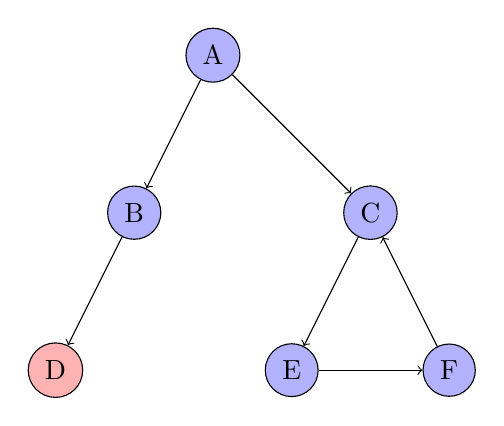
\begin{tikzpicture}
    \node[shape=circle,draw=black, fill = blue!30] (A) at (3,4) {A};
    \node[shape=circle,draw=black, fill = blue!30] (B) at (2,2) {B};
    \node[shape=circle,draw=black, fill = blue!30] (C) at (5,2) {C};
    \node[shape=circle,draw=black, fill = red!30] (D) at (1,0) {D};
    \node[shape=circle,draw=black, fill = blue!30] (E) at (4,0) {E};
    \node[shape=circle,draw=black, fill = blue!30] (F) at (6,0) {F};

    \draw[->] (A) -- (B);
    \draw[->] (A) -- (C);
    \draw[->] (B) -- (D);
    \draw[->] (C) -- (E);
    \draw[->] (E) -- (F);
    \draw[->] (F) -- (C);
  \end{tikzpicture}
  \caption{A graph for depth-first search. The result of $f$ on a vertex and its successors is denoted by the color. Red denotes an error and blue denotes ok.}
  \label{fig:dfsSetProblem}
\end{figure}

\begin{example}
  Suppose we start \dfsstep on the vertex $A$ in the graph depicted in \cref{fig:dfsSetProblem}. Additionally, suppose that the set of visited vertices is $\{B,C,D,E,F\}$. 
  
  As $A$ is not yet visited, we start the exploration process by evaluating $f$ on $A$ and its successors and as seen by the color this evaluates to ok. We have not seen any of the vertices before and therefore call \dfsstep on $B$ and $C$ and it returns ok, since $B$ and $C$ are already in the set of visited vertices. Therefore the function in total returns ok for $A$.

  This is however not what we expect it to do. $A$ can reach the vertex $D$ on which $f$ evaluates to an error and it can reach the cycle $[C,E,F,C]$. These wrong evaluations occured, because we assumed in the implementation that the visited set reports this property truthfully. Therefore we require this in every proof. If we would run this with an empty set of already visited vertices, then we gain the expected result.
\end{example}

\begin{definition}
  Let $a$ be a vertex in a graph $G$ and \lstinline|f: A → List A → Except String Unit| be a function. We say that $a$ has the \textit{DfsStepSemantics} property if $a$ does not reach a cycle in $G$ and every vertex reachable from $a$ in $G$ evaluates to ok on $f$ with its successors.
\end{definition}

This statement allows us to state the theorem we want to prove for \dfsstep more succintly.

\begin{theorem}[\dfsstepsematics]
  Let $\vec{v}$ be the input arguments with the vertex $a$ and visited set $V$. If every element in $V$ has the DfsStepSemantics property, then \dfsstep $\vec{v}$ returns ok iff $a$ has the DfsStepSemantics property.
\end{theorem}

We will prove this statement by induction on the amount of vertices not covered by the current walk, i.e. \lstinline|(List.toFinset G.vertices \ List.toFinset currWalk)|, for arbitrary walks and sets of visited vertices. We note that the base case is always true, because if this is equal to zero, then every vertex of $G$ is in the current walk. In $\vec{v}$ we have however explicit proofs that $a$ is a vertex in $G$ and that $a$ is not in the current path, so that we have a contradiction. The interesting case is therefore only the induction step. There we need a criteria for when \foldlexceptset returns an error.

In general, this seems hard to do.\todo{Think of an example}.
Here we already see that the set of visited vertices plays no really important role in the result of the statement as long as all elements in it have the DfsStepSemantics property. As long as we preserve this property in creating the sets we can view \foldlexceptset as individual calls when considering whether it returns an error or not.

\begin{lemma}[\foldlexceptsetisok]
  Let $l$ be a list of type $A$ and $S$ be a hash set of type $B$. Consider a property $p: B \to$ \lstinline|Prop| and a function \lstinline|f: A → HashSet B → (Except String (HashSet B))|, that fulfills the following two properties.
  Firstly, that $f$ preserves $p$, i.e. if every element in $S$ has the property $p$ and $f$ returns for the input $a$ and $S$ a set $S'$, then also every element in $S'$ has the property $p$.

  Secondly, that $f$'s acceptance status does not change on sets whose elements fulfill the property $p$, i.e. for any hash sets $S_1, S_2$ such that all elements in each hash set fulfill the property $p$, we have that for any element $a$ $f\ a\ S_1$ returns ok iff $f\ a\ S_2$ returns ok.
  
  Then there exists a hashset $S'$ that \foldlexceptset $f$ $l$ $S$ returns $S'$ iff $f a' S$ returns ok for any element $a'$ in $l$.
\end{lemma}
\begin{proof}
  We prove this by induction on the structure of $l$ for arbitrary $S$.

  If $l$ is empty \foldlexceptset always returns ok and there are no elements in $l$ so that the claim holds.

  If $l$ has the shape $hd::tl$, then $f hd init$ must return a set $S$. If not then \foldlexceptset returns an error and there is an element $a$ from $l=hd::tl$ for which $f a init$ is false so that both sides are false which finishes the prove.

  The remaining result of \foldlexceptset is therefore \lstinline|foldl_except_set f tl S|. From the induction hypothesis we know that then any element $a$ from $tl$ we have that $f a S$ returns ok. We already have the required result for $hd$, it remains to get that always $f\ a\ init$ returns ok. Since $f$ preserves $p$ and any element in $init$ had the property $p$, also any element in $S$ has the property $p$. Therefore we can use the second requirement for $f$ to conclude that  $f\ a\ init$ returns true for any element $a$ from $hd::tl$.
\end{proof}

The property in our case is the DfsStepSemantics property. The first requirement will follow from the induction hypothesis. Therefore it remains to show that \dfsstep preserves the DfsStepSemantics property. 

\begin{lemma}
  Let the 
\end{lemma}

\subsection{HashSets for depth-first search}

In the previous section, we used hash sets in the implementation of depth-first search. This offered a massive performance improve in practice in contrast to finite sets based on lists we used earlier. Unfortunately, while many lemmas for finite sets exist, there are currently almost no lemmas for hash sets. We try to bridge this gap partially by proving the correctness of insertion for hash sets.

\begin{lstlisting}
    lemma (.\StdHashSetcontainsinsert.) {S: HashSet A} (a:A ): 
    ∀ (a':A), (S.insert a).contains a' ↔ S.contains a' ∨ a = a' 

\end{lstlisting}